\section{Application to Sports}

\begin{frame}{The data}

	\textbf{Basketball game play-by-play data}

	\medskip

	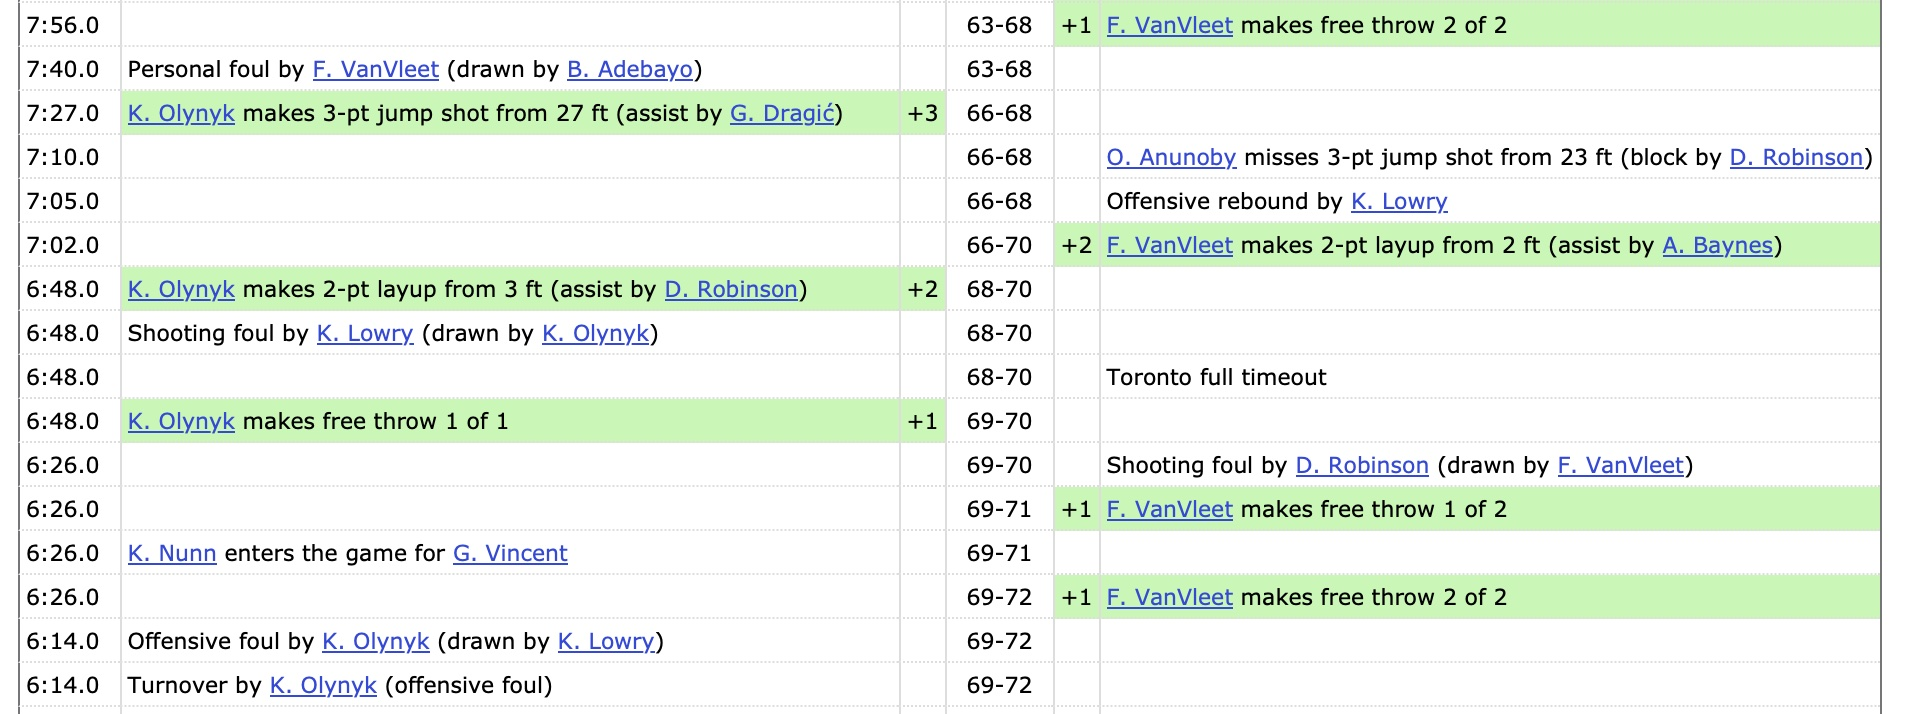
\includegraphics[width = \textwidth]{bbref-play-by-play.jpg}

	\medskip

	Miami Heat v. Toronto Raptors (January 20, 2021)
\end{frame}

\begin{frame}{Sequence modeling}

	How do we get this into a format that we can feed into a neural network?

	\pause

	\begin{center}
		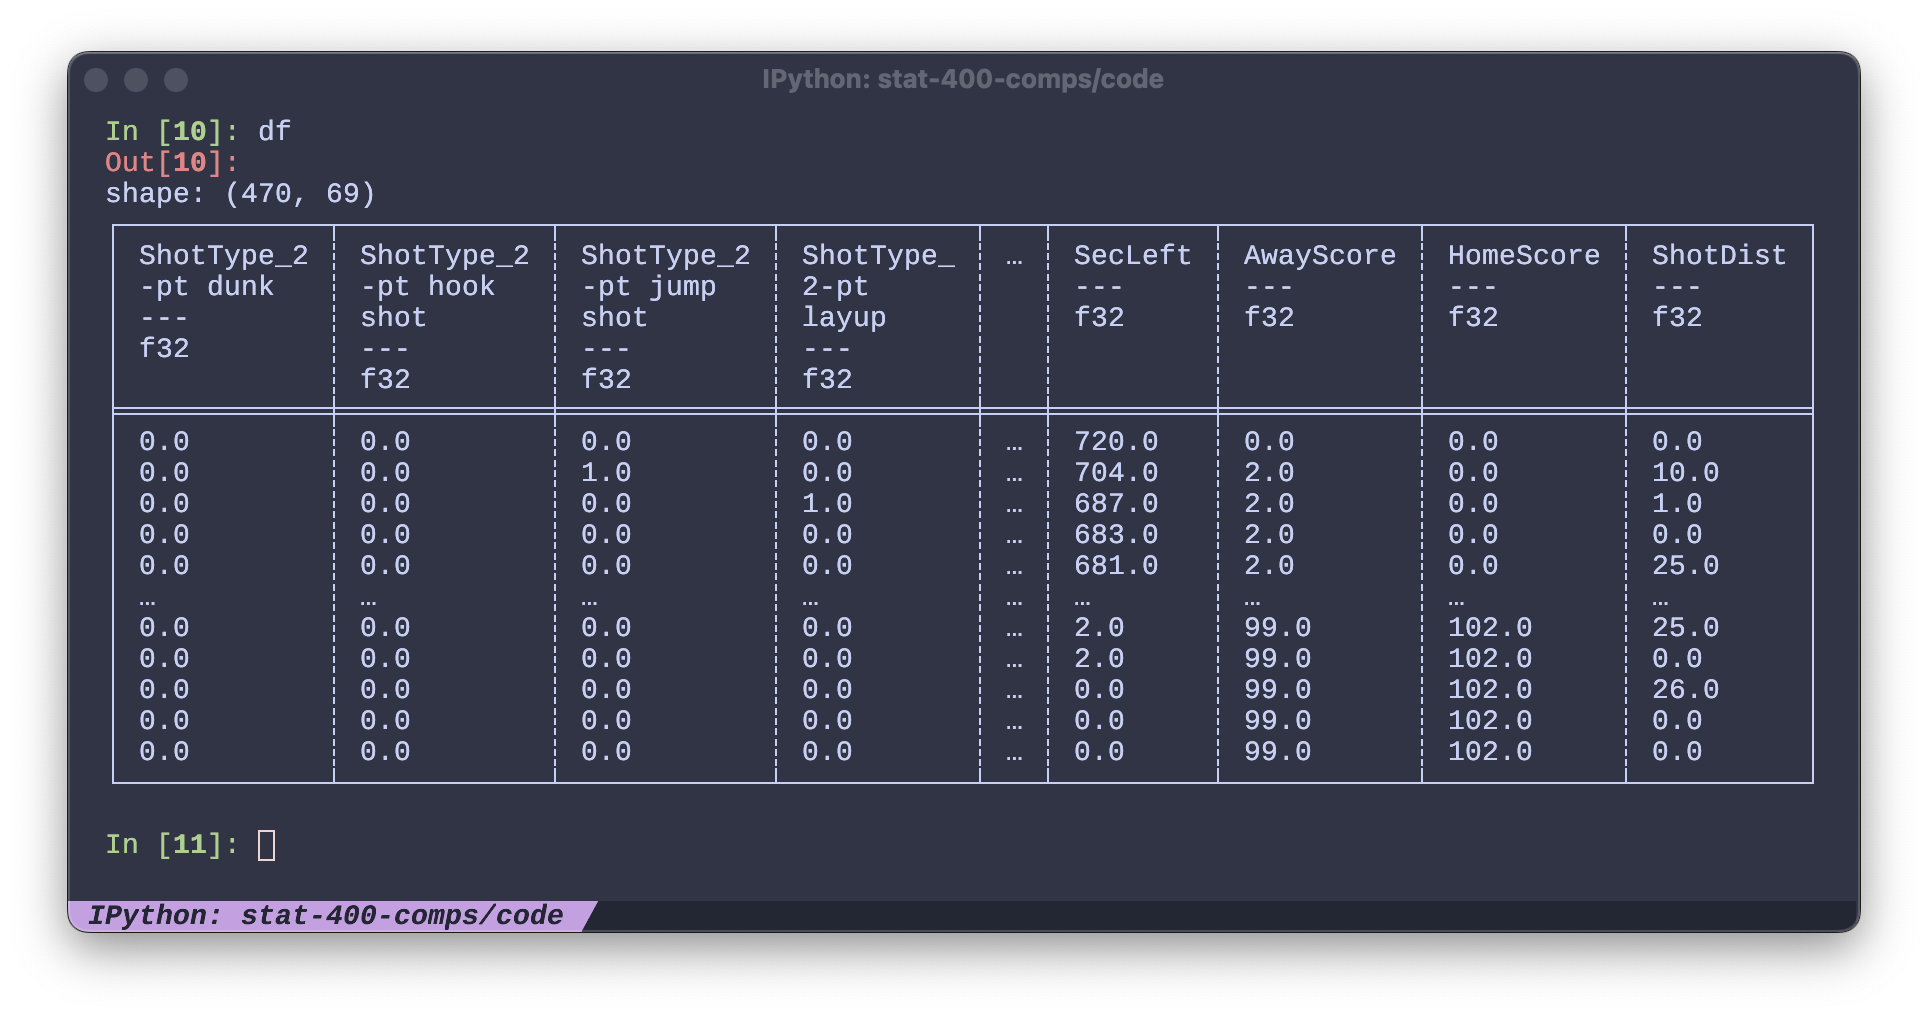
\includegraphics[width = \textwidth]{play-by-play-encoding.png}
	\end{center}

\end{frame}

\begin{frame}[t]{Recurrent Neural Networks}
	\begin{itemize}[<+->]
		\item $x_t$: event at time $t$
		\item $p_t$: win probability for home team at time $t$
		\item $h_t$: state of the game at time $t$
	\end{itemize}

	\medskip \pause

	\begin{center}
		\begin{tikzpicture}[
				every node/.style={font=\small},
				node distance = 1.5em,
				->,
			]
			\node (xt) {$x_t$};

			\pause

			\node[
				below = of xt, draw, rounded corners,
				inner sep=10pt, outer sep=5pt
			] (rnn) {RNN};

			\node[left = of rnn] (htm1) {$h_{t-1}$};

			\draw (xt) -- (rnn);
			\draw (htm1) -- (rnn);

			\pause

			\node[below = of rnn] (at) {$h_t$};

			\node[right = of rnn] (ht) {$h_t$};

			\draw (rnn) -- (ht);
			\draw (rnn) -- (at);

			\pause

			\node[below = of at] (pt) {$p_t$};
			\draw (at) -- (pt);
		\end{tikzpicture}
	\end{center}
\end{frame}

\begin{frame}[t]{RNNs (cont.)}

	\begin{itemize}
		\item $x_t$: event at time $t$
		\item $p_t$: win probability for home team at time $t$
		\item $h_t$: state of the game at time $t$
	\end{itemize}

	\pause

	\begin{center}
		\begin{tikzpicture}[
				every node/.style={font=\small},
				node distance = 1.5em and 2em,
				->,
				rnn/.style={ draw, rounded corners,
						inner sep=10pt, outer sep=5pt},
				every edge quotes/.style={below, font=\tiny},
			]

			\node[rnn] (rnn1) {RNN};
			\node[rnn, right = of rnn1] (rnn2) {RNN};
			\node[rnn, right = of rnn2] (rnn3) {RNN};
			\node[right = of rnn3] (rnn4) {$\cdots$};

			\node[left = of rnn1] (h0) {$h_0$};

			\node[above = of rnn1] (x1) {$x_1$};
			\node[above = of rnn2] (x2) {$x_2$};
			\node[above = of rnn3] (x3) {$x_3$};

			\node[below = of rnn1] (h1) {$h_1$};
			\node[below = of rnn2] (h2) {$h_2$};
			\node[below = of rnn3] (h3) {$h_3$};

			\node[below = of h1] (p1) {$p_1$};
			\node[below = of h2] (p2) {$p_2$};
			\node[below = of h3] (p3) {$p_3$};

			\draw (h0) -- (rnn1);
			\draw (rnn1) edge["$h_1$"] (rnn2);
			\draw (rnn2) edge["$h_2$"] (rnn3);
			\draw (rnn3) edge["$h_3$"] (rnn4);

			\draw (x1) -- (rnn1);
			\draw (x2) -- (rnn2);
			\draw (x3) -- (rnn3);

			\draw (rnn1) -- (h1);
			\draw (rnn2) -- (h2);
			\draw (rnn3) -- (h3);

			\draw (h1) -- (p1);
			\draw (h2) -- (p2);
			\draw (h3) -- (p3);
		\end{tikzpicture}
	\end{center}
\end{frame}

\begin{frame}{Training}
	\begin{itemize}[<+->]
		\item Implemented using the \texttt{pytorch} Python library.

		      \medskip

		\item Trained on $3,040,524$ events across $6,600$ NBA games using binary cross-entropy loss.

		      \medskip

		\item Tested a variety of different models
		      \begin{itemize}
			      \item dimension of hidden state $h_t$
			      \item different models for computing $p_t$ from $h_t$
			      \item different forms of RNNs (LSTM, GRU)
		      \end{itemize}
	\end{itemize}
\end{frame}

\begin{frame}{How'd we do?}
	\textbf{The good news:}
	\begin{itemize}
		\item Our RNN gets 73 percent accuracy!
	\end{itemize}

	\bigskip \pause

	\textbf{The bad news:}
	\begin{itemize}
		\item Picking the current leader gets 73 percent accuracy...
	\end{itemize}

	\bigskip \pause

	\textbf{Implications:}
	\begin{itemize}
		\item Our model learned to just pick the currently-winning team.
		      \note{(More on this in the paper)}
	\end{itemize}
\end{frame}

\begin{frame}{Why did this happen?}
	\begin{enumerate}[<+->]
		\item Score \emph{is} the best predictor the winner.
		\item The model isn't appropriate.
		\item I don't know what I'm doing.
	\end{enumerate}
\end{frame}

\begin{frame}{Next steps}
	\textbf{Other sports}

	\begin{itemize}
		\item Less scoring in hockey and soccer--score caries less information?
		      \note{if we think about shots and chances as random events, sports that score}
	\end{itemize}

	\pause \bigskip

	\textbf{Incorporate player information}

	\begin{itemize}
		\item Steph Curry taking a shot is different from Markelle Fultz
		\item Side effect: player and/or team embeddings?
	\end{itemize}

	\pause \bigskip

	\textbf{Different network architecture}

	\begin{itemize}
		\item Smarter pre-/post-processing?
		\item Stacking RNN layers?
		\item Transformer?
	\end{itemize}
\end{frame}
